% Section 7: Results
\newcommand{\stc}[1]{\hbox to 2.5em{{#1}\hfil}}

\section{Results}

\subsection{Summary of Runs} \label{sec:recsummary}

Much as with DC2, we executed numerous but short pipeline runs over
a sampling of the data from the CFHT-LS fields D3 and D4 and from the
simulated data collections, SimDeep and SimWide.  These short runs
were used to do initial debugging, performance analysis, and quality
analysis which resulted in numerous bug fixes and important algorithm
optimizations.  These short runs also allowed us to explore different
policy parameter settings to understand the trade off between data
quality and performance.  

For our final, detailed analysis of the data quality and processing
performance, we focused on two productions runs with identical
versions of the software and configuration: {\tt rlp1233} and {\tt
rlp1234}.  These two runs
processed different subsets of the focal plane for 85 visits to the
CFHT-LS D3 on our own LSST cluster.  These visit were selected based
on the availability of the calibration data needed to calibrate raw
science images.  The Image Processing and Source Detection (IPSD)
pipeline featured 1 master pipeline and 31 slice processes running
across four nodes of the cluster (thus each run processed 31 amplifier
images in parallel).  The Association pipeline (ap) ran on node 10
within one master process and one slice process.  The ``NightMOPS''
pipeline (part of the Moving Objects Prediction System) ran on node 9
with 1 master process and 5 slice processes.  Taking a lesson from
DC2, we did not use any of the ``slower'' cluster nodes (nodes 1-4)
for pipeline processes as they would have pulled down the over
performance of the pipeline.  We note that we had other infrastructure
processes on the cluster nodes running which did not interfere
noticeably with the pipeline processes.  Node 4 (which did not have
any pipeline processes on it) hosted the event broker process, and
node 9 (which had extra unused processor cores available) hosted the
event monitor which loaded logging events into the database.

\begin{table}[htbp]
\begin{center}
\caption{The stages comprising the IPSD pipeline
\label{tbl:ipsdstages}}
\small
\vspace{\baselineskip}
\begin{tabular}{rrl|rrl}
\hline\hline
\# &\multicolumn{1}{l}{Type$^a$}& Name      & \# &\multicolumn{1}{l}{Type$^a$} & Name   \\ 
\hline
 1 &         &                    sliceInfo & 24 &\stc{FDO}& rawImageAndMetadataOutput1 \\
 2 &         &                      symLink & 25 &*\stc{S} &                       isr1 \\
 3 & \stc{FI}&                  imageInput0 & 26 &*\stc{DI}&            wcsSourcesInput \\
 4 & \stc{DI}&               visitMetadata0 & 27 &*\stc{S} &           wcsDetermination \\
 5 &         &           transformMetadata0 & 28 &*\stc{FO}&  calibratedExposuresOutput \\
 6 &         &            validateMetadata0 & 29 &*\stc{}  &           CcdMetadataStage \\
 7 & \stc{FO}&         visitMetadataOutput0 & 30 &*\stc{FI}&      templateMetadataInput \\
 8 &\stc{FDO}&   rawImageAndMetadataOutput0 & 31 &*\stc{}  &          templateDimension \\
 9 &*\stc{}  &  identifyCalibrationProducts & 32 &*\stc{}  &               templateBBox \\
10 &*\stc{FI}&             calibrationInput & 33 &*\stc{FI}&      templateSubimageInput \\
11 &         & transformCalibrationMetadata & 34 & \stc{FO}&     templateSubimageOutput \\
12 &*\stc{S} &                         isr0 & 35 &*\stc{S} &           imageDifference0 \\  
13 &*\stc{S} &              sourceDetection & 36 &*\stc{S} &           imageDifference1 \\  
14 & \stc{FO}&   calibAndBkgdExposureOutput & 37 &*\stc{FO}&      differenceImageOutput \\
15 &*\stc{S} &            sourceMeasurement & 38 &*\stc{S} &               addAndDetect \\  
16 &*\stc{FDO}& exposureAndWcsSourcesOutput & 39 &*\stc{S} &       diaSourceMeasurement \\
17 &*\stc{S} &             psfDetermination & 40 &*\stc{}  &          sourceToDiaSource \\  
18 & \stc{FO}&                    psfOutput & 41 &*\stc{S} &       sourceClassification \\
19 & \stc{FI}&                  imageInput1 & 42 &*\stc{DO}&           diaSourceOutput0 \\
20 & \stc{DI}&               visitMetadata1 & 43 &*\stc{DO}&           diaSourceOutput1 \\
21 &         &           transformMetadata1 & 44 &*\stc{}  &           associationEvent \\
22 &         &            validateMetadata1 & 45 &*\stc{DO}&                sdqaOutput0 \\
23 & \stc{FO}&         visitMetadataOutput1 & 46 &*\stc{DO}&                sdqaOutput1 \\
\hline
\multicolumn{6}{l}{$^a$Stage Type codes: S = scientific algorithm, * = necessary for production mode,} \\
\multicolumn{6}{l}{\phantom{$^a$Stage Type codes:} F = File I/O, D = Database I/O, I = Data Input, O = Data Output} \\
\end{tabular}
\end{center}
\end{table}

\begin{table}[hbtp]
\begin{center}
\small
\caption{The stage comprising the Association and NightMOPS pipelines
\label{tbl:otherstages}}
\vspace{\baselineskip}
\begin{tabular}{rrl|rrl}
\hline\hline
\multicolumn{3}{c|}{Association} & \multicolumn{3}{c}{NightMOPS}  \\
\# & \multicolumn{1}{l}{Type$^a$}& Name & \# & \multicolumn{1}{l}{Type$^a$}& Name  \\ 
\hline
 1 &         & symLink                  &  1 &*\stc{S} & NightMopsStage \\ 
 2 &*\stc{DI}& load                     &  2 &*\stc{DO}& output         \\ 
 3 &*\stc{DI}& diaSourceInput           &  3 &*\stc{}  & associationEvent  \\ 
 4 &*\stc{S} & MatchDiaSourcesStage     &  && \\ 
 5 &*\stc{DO}& diaSourceMatchOutput     &  && \\ 
 6 &*\stc{DI}& predInput                &  && \\ 
 7 &*\stc{S} & MatchMopsPredsStage      &  && \\ 
 8 &*\stc{DO}& predMatchAndObjectOutput &  && \\ 
 9 &*\stc{DO}& store                    &  && \\ 
\hline
\multicolumn{6}{l}{$^a$Stage Type codes: S = scientific algorithm, * = necessary for production mode,} \\
\multicolumn{6}{l}{\phantom{$^a$Stage Type codes:} F = File I/O, D = Database I/O, I = Data Input, O = Data Output} \\
\end{tabular}
\end{center}
\end{table}


One of the intended goals of the DC3a was exercise the use of the
parallel filesystem, Lustre, we installed on the LSST cluster.  Much
as with DC2, we found Lustre to be fairly unstable under heavy IO,
apparently causing catastrophic failure of the filesystem.  This may
have been due to an insufficient number of fileserver nodes for the
level of IO we were attempting; however, schedule and hardware
resource limitations prevented our exploring the causes in any
detail.  Consequently, the final runs were conducted using NFS-mounted
filesystems (which are known to perform poorly under most conditions).  

Ultimately, the simulated data was not used as part of the final
analysis.  While the two simulated collections were instrumental
in understanding and correcting processing problems, we found that the
quality of the template images were insufficient for producing useful
difference images and database results.  

In addition to the runs on our own LSST cluster, we also conducted
runs on the NCSA Abe cluster.  The purpose of these runs were to
explore the scalability of the pipeline processing up to higher
numbers of slices.  In particular, we have executed runs that process
entire CFHT focal plane exposures simultaneously.  This was done by
running the IPSD pipeline on Abe with 288 slice processes across 36
8-core nodes.  While Image I/O was carried out using the Lustre
filesystem attached to that platform, database I/O occurred with the
database residing on the LSST cluster ({\tt lsst10}).  

DC3a schedule constraints limited the detailed analysis
that could be completed for this report; nevertheless, we see that the
pipeline scaled fairly well at this level.  In \Sec{sec:timing} we
present and discuss comparisons between the ``narrower'' (fewer
slices) but longer (more visits) runs on the development cluster with
the wider but shorter run on Abe.  The Abe run was only able to
complete twelve visits before suffering a disabling failure.  This was
caused by a failure in the event system when the broker run up against
an operating system limit on the number of simultaneously open file
descriptors (1024 by default).  Considering the large number of slices
times a few event channels, it was clear that we were operating on the
edge of this limit.  Raising this limit appears to correct the
problem, and we expect to proceed with larger (both wider and longer)
runs in the early days of DC3b.  

These Abe runs provided important qualitative accomplishments:

\begin{itemize}
\item They revealed configurable system limits that must be increased:
\begin{itemize}
\item the event broker must support over 1000 simultaneous open file
  descriptors (discussed above), and 
\item the MySQL database must support $\gtrsim$ 300 simultaneous
  connections.  
\end{itemize}
\item We demonstrated the integration of grid-based job management
  (via Condor-g) into our orchestration layer
\item we demonstrated the successful use of the parallel Lustre
  filesystem.  
\end{itemize}

In summary, Table \ref{tbl:runsummary} lists the pertinent
production runs and the data processed which form the primary basis
for our results analysis.  A discussion of the performance results
for both the Abe run and the runs on the development cluster appear in
section \ref{sec:timing}.  In the next section, we assess the
scientific and algorithmic results of the processing, focusing
specifically on the development cluster.  

\begin{table}[htbp]
\centering
\caption{Summary of Production Runs analyzed in this report
\label{tbl:runsummary}}
\vspace{\baselineskip}
\begin{tabular}{rccccc}
\hline\hline
          &         &       & \multicolumn{3}{c}{Images Processed: Num/Size} \\
runId     & nVisits & nAmps & Raw Images & Ancil. Images & Output Images \\ \hline
rlp1233   & 85      & 31  & 5146/24 GB    & 88/13 GB       & 60525/240 GB \\ 
rlp1234   & 85      & 31  & 5146/24 GB    & 88/13 GB       & 60525/240 GB \\ 
rlpabe041 & 12      & 288 & 3456/33 GB    & 15/2 GB        & 79368/313 GB \\ \hline
Total     & ---     & 250 & 13748/81 GB   & 191/28 GB      & 200418/793 GB \\ \hline
\end{tabular}
\end{table}


\subsection{Science Data Quality}
We chose several areas for which to assess the scientific data quality of the DC3a outputs:
\begin{itemize}
\item Cosmic ray rejection
\item WCS accuracy
\item Difference image quality
\item Difference image lightcurve quality
\item Recovery of known solar system objects
\end{itemize}
Other areas could of course be added to this list, but the ones chosen
are judged to be the most demanding for the software system to meet,
and are each directly related to science requirements. 
\paragraph{Cosmic Ray Rejection}
The DC3a processing flow contains two methods of rejecting cosmic
rays, that can be used as alternatives or in tandem.  For the DC3a
reference runs, the two methods were used in tandem.
\begin{itemize}
\item As presented in section \ref{sec:isr}, the ISR detects and
  interpolates over cosmic rays in individual images
\item The Association Pipeline (AP) makes use of the two exposures per
  visit organization of the survey to discriminate against cosmic
  rays.  A positive flux DIASource present in only a single exposure
  of a visit will be considered a cosmic ray.
\end{itemize}
Quantitative analysis of the ISR cosmic ray rejection analysis method
has been performed by comparing the number of pixels affected by
synthetic cosmic rays in each exposure 1 with the number identified as
cosmic rays by the ISR.  The fraction successfully identified is
nearly 100\% for rlp1233.  Analysis of the performance of the AP based
method has proven to be difficult when run in tandem with the ISR
method, and will require a separate set of runs with the ISR method
turned off.  The joint analyis will lead to an optimized cosmic ray
rejection technique for DC3b.

\paragraph{WCS Accuracy}
The WCS determination algorithm is implemented as part of the Image
Processing and Source Detection pipeline (IPSD) and is discussed in
section \ref{sec:wcs}.  The achieved WCS accuracy is crucial for
subsequent processing, especially for production of difference images.
The procedure used to assess the WCS accuracy is as follows:
\begin{itemize}

\item A set of exposures from visits processed by a particular run is
  picked for analysis. For each exposure:
\begin{enumerate}
\item The WCS\_Sources identified by the ICP for WCS determination are retrieved from the
  science database for the run.
\item The pixel coordinates for each WCS\_Source are converted from
  ccd coordinates to amplifier coordinates, and are input to the
  wcstools program ``xy2sky'' along with the corresponding amplifier
  science image to yield predicted sky coordinates for the
  WCS\_Source.
\item The star catalog used for WCS determination is searched for the
  predicted sky coordinates.  The distance between the predicted sky
  position and the nearest catalog object is recorded in an output file
\end{enumerate}
\item A histogram of the distances is calculated, and its properties
  used as metrics for WCS performance.
\end{itemize}

\begin{figure}[p]
\begin{center}
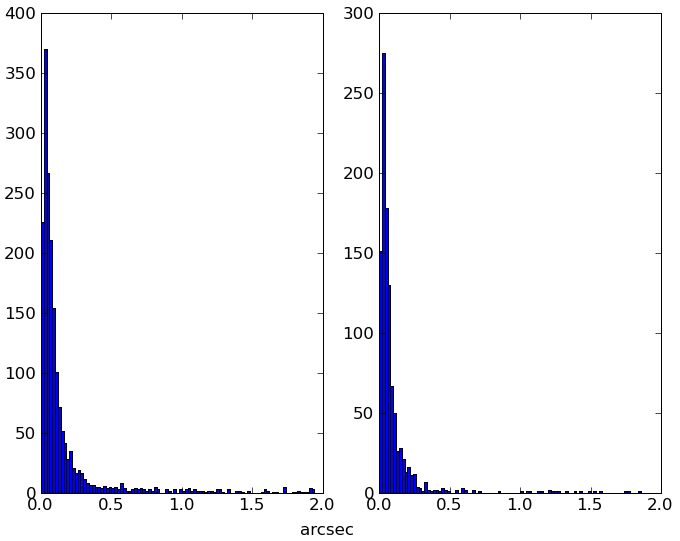
\includegraphics[height=3.35in]{images/rlp1233_1234_match.png}
\caption{Histogram of the distances between positions predicted from WCS, and
  true catalog positions for rlp1233/695833-e0 on the left and
  rlp1234/696554-e0 on the right}  
\label{fig:wcs1}
\end{center}
\end{figure}

\begin{figure}[p]
\begin{center}
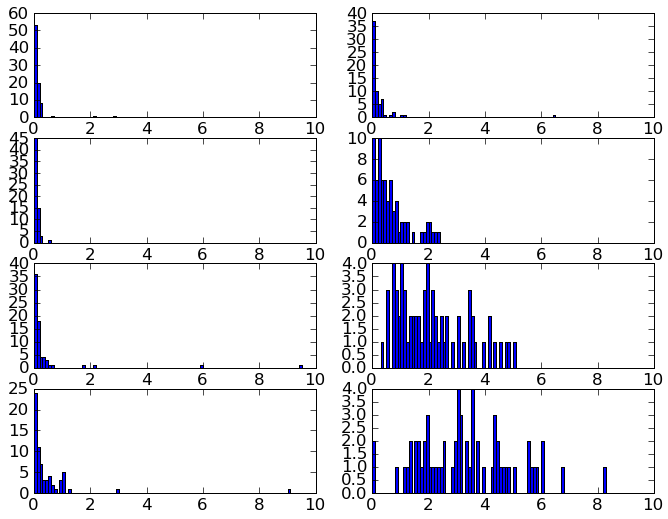
\includegraphics[height=3.35in]{images/rlp1233_ccd1_match.png}
\caption{Histogram of the distances between positions predicted from WCS, and
  true catalog positions for rlp1233/695833-e0, showing the individual
amplifiers from ccd1}  
\label{fig:wcs2}
\end{center}
\end{figure}

Figure \ref{fig:wcs1} shows the resulting histograms for typical
exposures from runs rlp1233 (visit 695833-e0) and rlp1234 (visit
696554-e0). Both histograms show very similar behavior, with the peak
of the histogram around 30 mas, about 0.2 pixel.  In both cases there
is a shallow tail that extends to large distances, beyond the plotting
limit in the figure.  Figure \ref{fig:wcs2} shows that the tail is
far more significant than is initially apparent, since it
results from very poor wcs fits that are confined to individual
amplifiers.

\begin{figure}[tbh]
\begin{center}
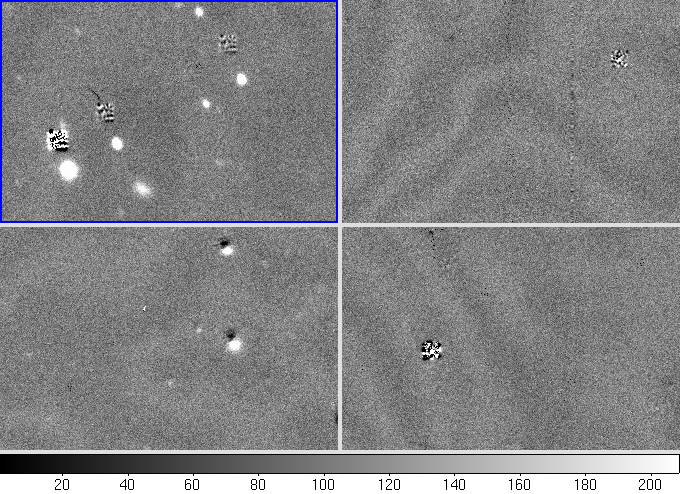
\includegraphics[width=6in]{images/rlp1233_v695833-e0-c001-mosaic.png}
\caption{A mosaic of different types of difference images, all from rlp1233/695833-e0-c001}  
\label{fig:diffim1}
\end{center}
\end{figure}

For DC3a purposes, we define WCS failure for an image to occur when
more than 50\% of the predicted WCS\_Source positions are in error by
more than 1 arcsec.  This is roughly the level beyond which the difference
image matching kernels can no longer compensate for image misalignments. With
this criterion, for run rlp1233 there were 109 failures out of 2629
images processeed, or 4\%.   For rlp1234 there were 14 failures out
of 2509 images processed, or 0.5\%.  It must be noted however, that
this criterion for WCS failure will need to be considerably stricter
for DC3b and beyond, because processing of image stacks for deep
detection and measurement, and the determination of astrometric models
all require much better WCS quality.

\paragraph{Difference Image Quality}

Visual inspection of DC3a difference images shows three distinct
categories. First, difference images produced from images with failed 
WCS's show either ``bipolar'' subtractions in the case of failures
near the cutoff criterion, or completely nonfunctional subtractions in
the case of extreme WCS failures.  Images with successful WCS's
generate subtractions that look good except in the vicinity of bright
stars,where a high spatial frequency pattern is evident.  Examples of
these three categories are shown in Figure \ref{fig:diffim1}.

In the remainder of this discussion, we leave aside the roughly 2\% of
the difference images that involved WCS failures, since they tell us
little about the performance of the difference image algorithm itself.
In the absence of variable or moving sources, an ideal difference
image will have a mean of zero, and show uncorrelated random
fluctuations at the level expected from the variance of the input
images.  We therefore define a ``figure of merit image'' as
\begin{equation}
f(x,y)~=~d(x,y)/\sqrt {v(x,y)}
\end{equation} 

where $f$ is the figure of merit, $d$ is the difference image, and $v$
is the predicted variance image.  A typical figure of merit image is
shown in Figure \ref{fig:diffim2}.  A plot along a horizontal line through
the subtracted bright star near the center of the image is shown in
Figure \ref{fig:diffim3}.  This plot shows several aspects of the difference
image quality:

\begin{itemize}
\item The average level of the image is near zero, as expected
\item Away from bright stars, the level of the noise is near 1.0, the
  expected value
\item In the footprint of bright stars, the noise is larger than
  expected by a large factor, about 20 in this particular case.
\end{itemize}  

\begin{figure}[p]
\begin{center}
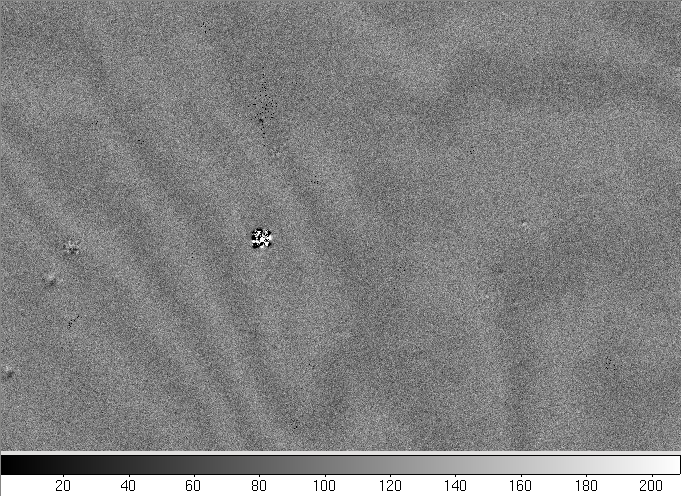
\includegraphics[height=3.25in]{images/rlp1233_v695833-e0-c001-a03-fom_img.png}
\caption{A figure-of-merit image for
  rlp1233/695833-e0-c001-a03}  
\label{fig:diffim2}
\end{center}
\end{figure}

\begin{figure}[p]
\begin{center}
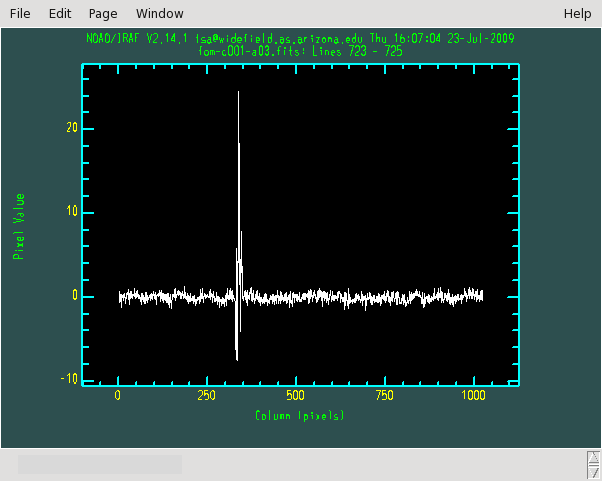
\includegraphics[height=3.25in]{images/rlp1233_v695833-e0-c001-a03-fom_plot.png}
\caption{Line section through figure-of-merit image for
  rlp1233/695833-e0-c001-a03.  The line is chosen to pass through the
  subtracted bright star at (338,725), which is near the center of the
image in Figure \ref{fig:diffim2}}  
\label{fig:diffim3}
\end{center}
\end{figure}

\paragraph{Difference Light Curve Quality}
Leaving out images that had WCS failures, run rlp1233 yielded 63000
objects with difference sources detected above threshold in at least
one visit. As Figure \ref{fig:lightcurve1} shows, the number of visits
for which difference sources were detected varies widely with the object, between 1 and
about 75.  The latter number is close to the number of visits
processed in rlp1233, which is 85.  Spot checking of these sources in
the images suggests that the vast majority are the result of artifacts
in the difference images, with residuals around bright stars being the
most frequent cause.  The highly structured nature of the difference
image residuals, combined with the relatively large kernel footprint,
causes further artifacts, since multiple peaks can be detected in a
single footprint.  In general, though it will certainly be the case
that real astrophysical signals from variable stars and transient
events are present in this data, it is currently impractical to
separate them from the noise with the analysis tools readily
available.

\begin{figure}[htb]
\begin{center}
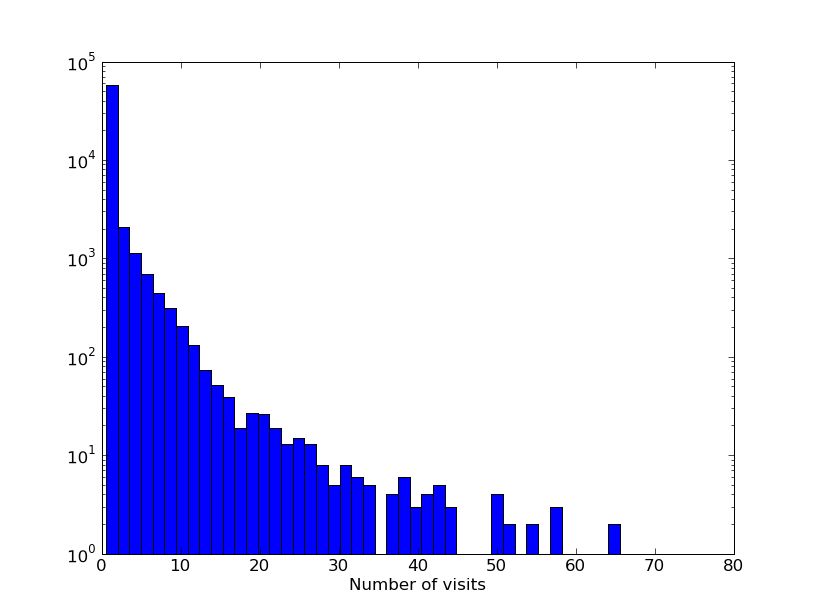
\includegraphics[height=3.25in]{images/rlp1233DiffLCHisto.png}
\caption{Histogram of number of Objects with DIASources in a given number of
  visits in rlp1233}  
\label{fig:lightcurve1}
\end{center}
\end{figure}

  
% \paragraph{Recovery of Known Solar system Objects}

\subsection{Timing Results}
\label{sec:timing}

As in DC2, we use the logging framework (in which every log message is
time-stamped) to instrument our pipeline processing code.  We can
calculate how much time is spent on the different contributors to the
overall processing time, including I/O, middleware overhead,
scientific processing.  

\begin{table}[ht]
\begin{center}
\caption{Average Processing Times Per Visit
\label{tbl:visitstats}}
\vspace{\baselineskip}
\begin{tabular}{ l | c | c }
\hline\hline
          & Total Processing Time, corrected
          & Application Processing Time \\ 
Pipeline  & average $\pm$  $3\sigma$ (s) & average $\pm$ $3\sigma$ (s) \\ \hline
IPSD      & 264.7 $\pm$ 20.2 & 264.1 $\pm$ 20.1  \\ 
nightmops & 10.6  $\pm$  4.4 & 0.174 $\pm$  4.4  \\ 
ap        & 1.4   $\pm$  0.7 & 0.021 $\pm$  0.7  \\ \hline
\hline
\end{tabular}

\end{center}
\end{table}


In Table \ref{tbl:visitstats}, we summarize the statistics for processing
a single visit through each pipeline.  For each quantity, the error
given represents the calculated $3\sigma$ variation of the
distribution of values.  The total time is corrected to remove the
time the pipelines spend waiting for data events to arrive.  For the
IPSD and nightmops pipelines, this is the time it waits for a new data
event to arrive.  As mentioned in section \ref{brokerprob}, we
throttled the time between to data events to match the expected visit
nnprocessing time to avoid having too many unconsumed data events pile
up in the event broker; this typically resulted in an extra 20-30
second wait for a data event before processing could resume.  The ap
pipeline, on the other hand, receives its initial event from the IPSD
pipeline; thus, it had to wait on average 4.4 minutes for the IPSD
pipeline to complete before it could do its work.

\begin{figure}[htbp]
\begin{center}
%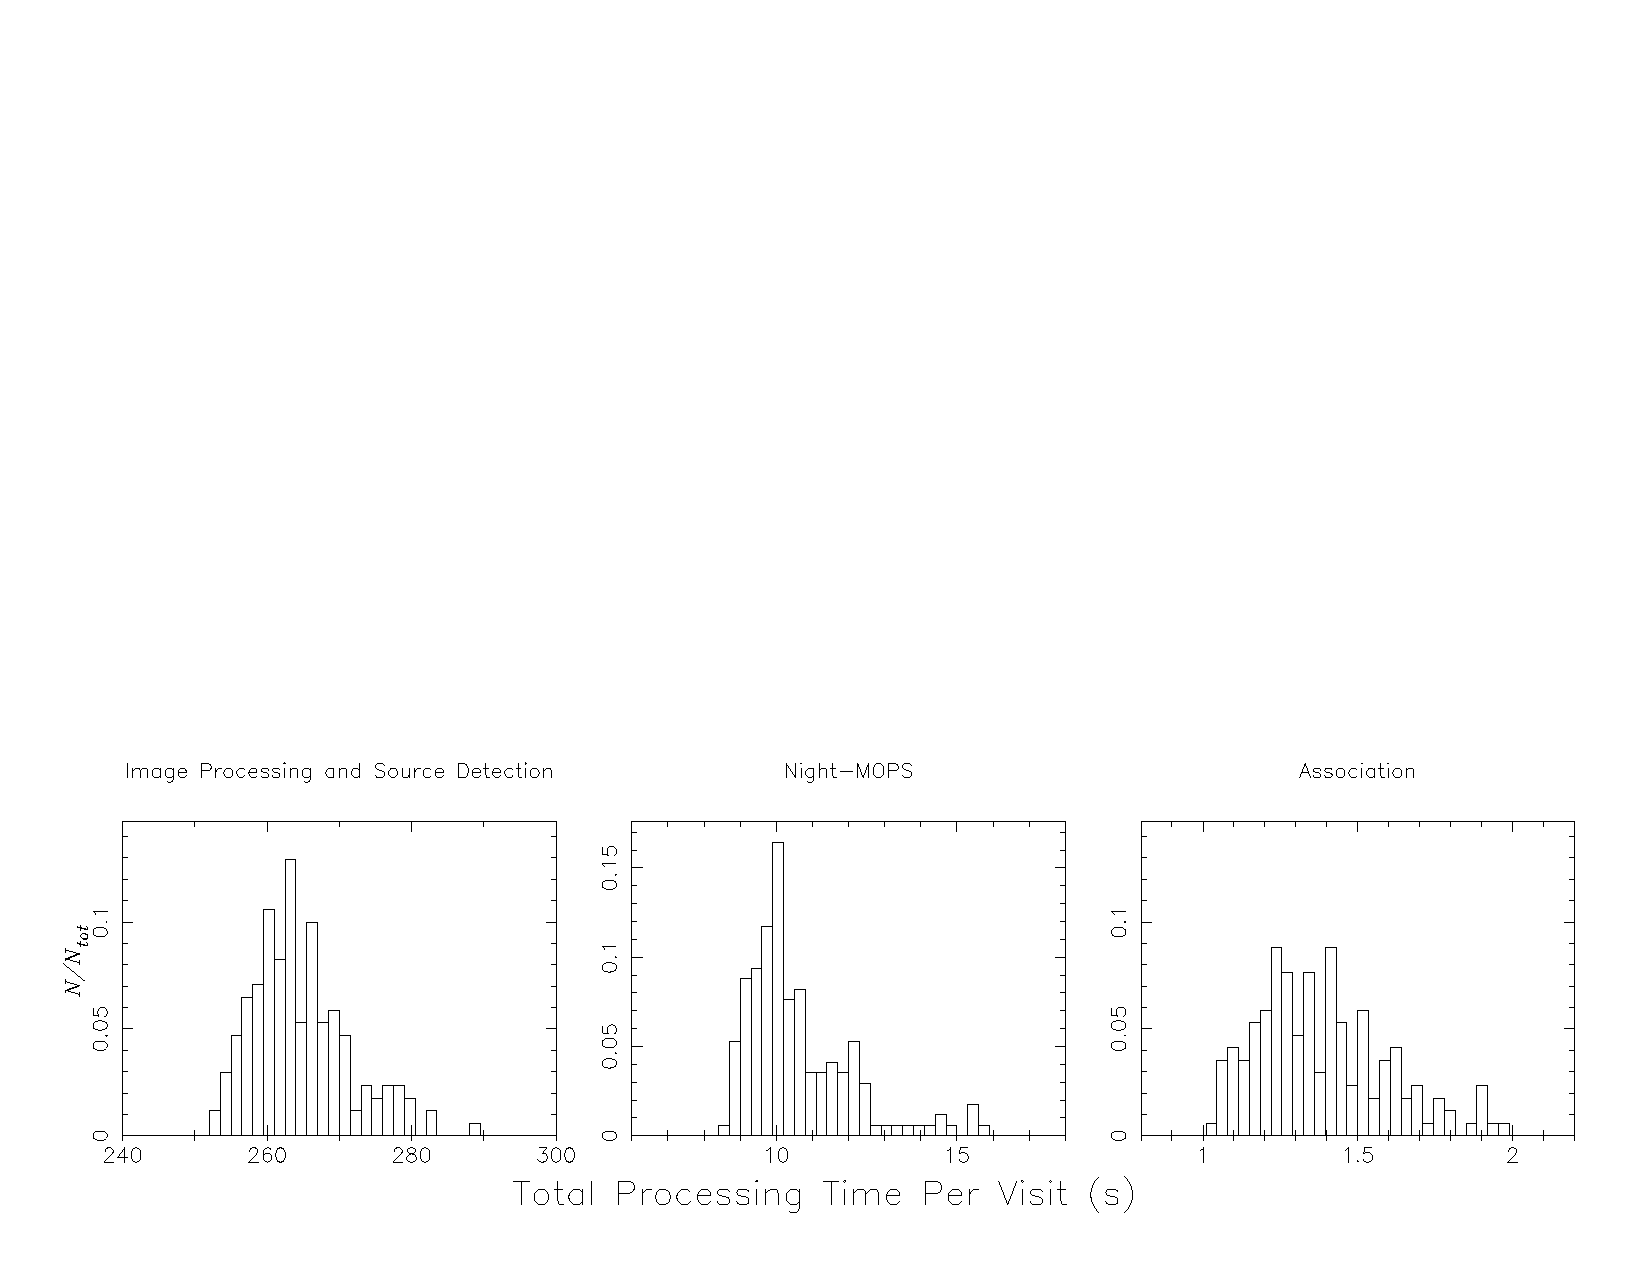
\includegraphics[width=\textwidth,bb=0 0 800 276,viewport=25 25 775 250,clip]{images/visitdist.pdf}
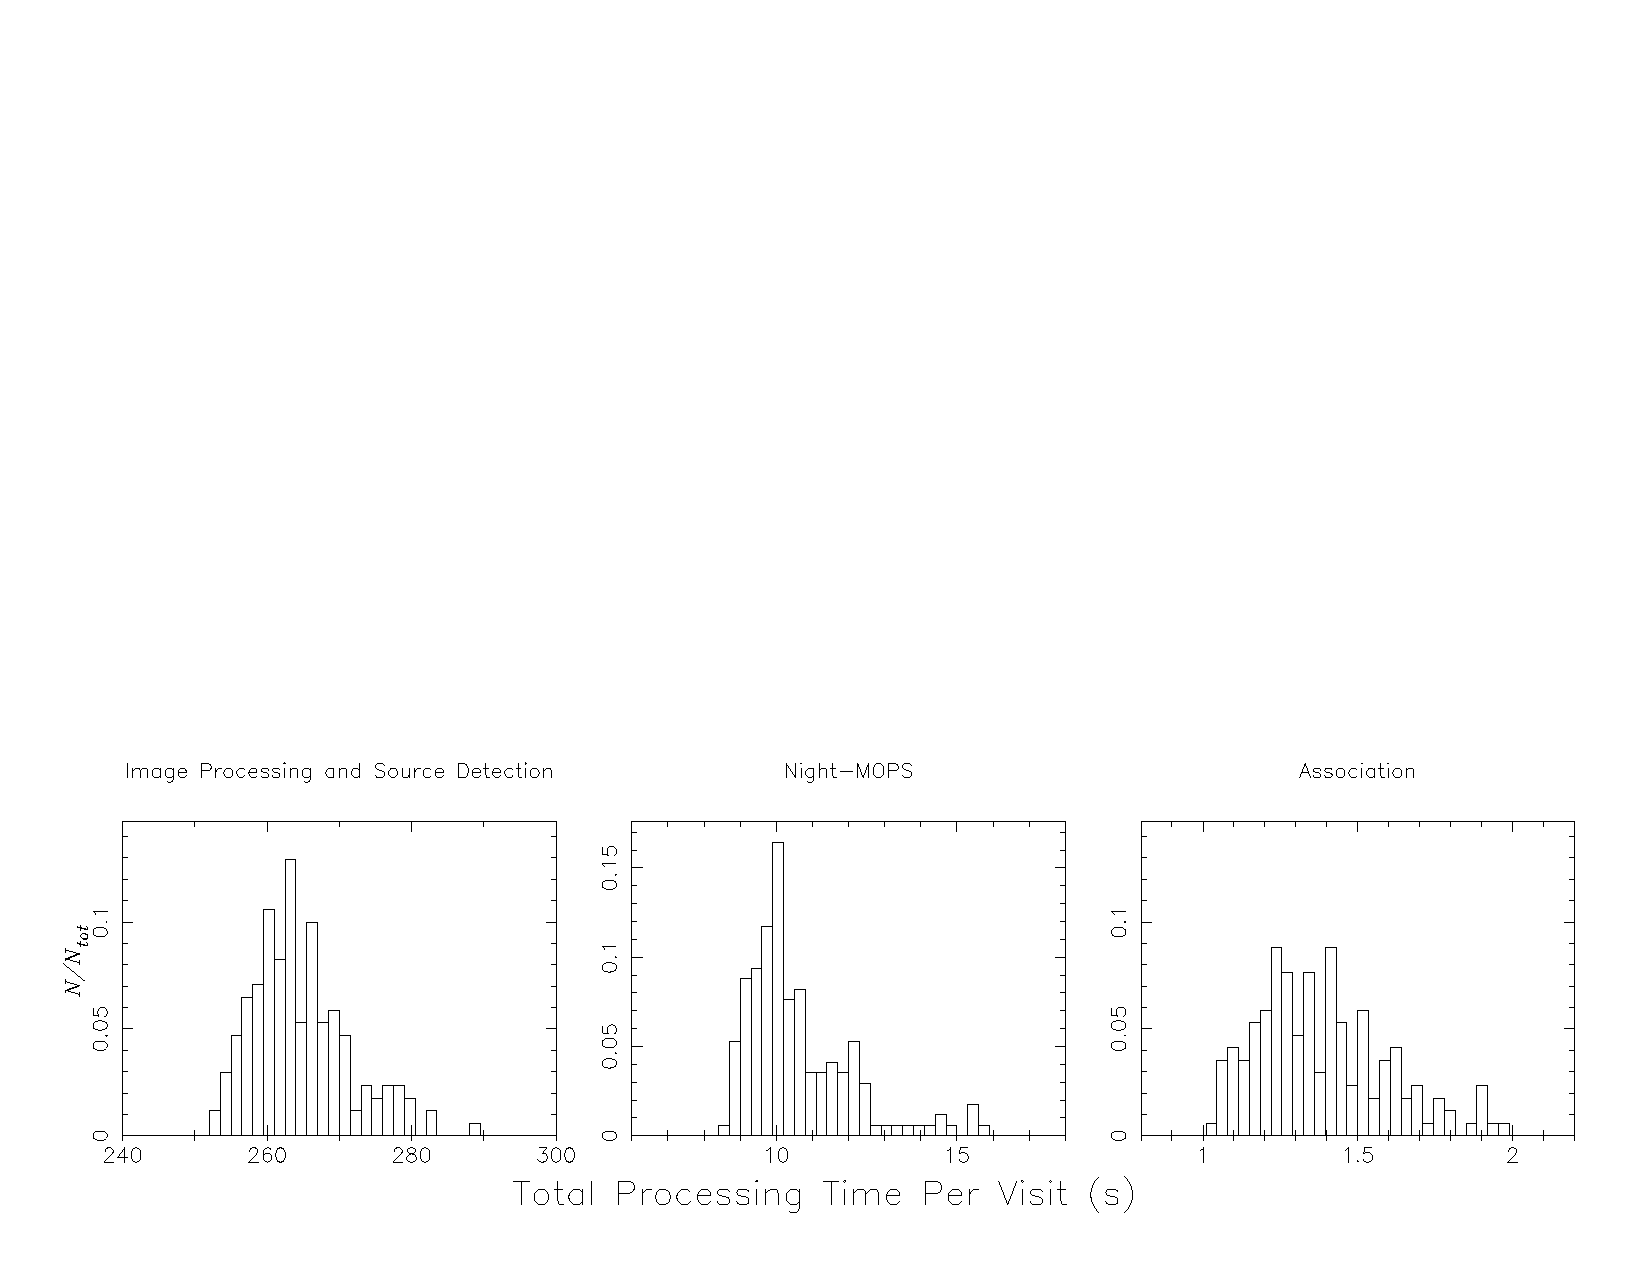
\includegraphics[width=\textwidth,bb=0 0 800 276,viewport=25 25 775 250,clip]{images/visitdist.pdf}
\caption{Histogram of the times to process each visit (not including
  time waiting on data events).  The $y$-axis measure the fraction of
  the 170 visits in each time bin.  
\label{fig:visitdist}}
\end{center}
\end{figure}


The ``Application Processing Time'' tallies on the time spent in total
by all the pipeline stages in their preprocess, process, and
postprocess functions where I/O is carried out and application
algorithms are applied.  (The times in these functions are included
only in cases where a stage actually provides an implementations for
them.)  It excludes the overhead by the pipeline framework for
managing the execution of the stages.  As the numbers show, the
pipeline adds very little to the processing time of a visit.  A more
precise analysis of the pipeline overhead is presented below.  

The variation in the processing is in general much smaller in DC3a as
it was in DC2: in the latter, the $3\sigma$ half-width was 108
seconds in the image processing pipeline, while we now have 20
seconds.  Furthermore as illustrated in Fig. \ref{fig:visitdist}, the
processing times do not feature the unexplained double-peaked
distributions we saw in DC2.  In summary, our we're getting much more
consistent processing times in DC3a than we did in DC2.  This has an
important impact on the overall performance because the total time
spent on a stage is driven primarily by the duration of the slice that
took the longest time.  

Tables \ref{tbl:scistagetimes} --- \ref{tbl:otherstagetimes} list
the average time spent in actual {\it application code} each stage for
each pipeline.  (That is, these include the time spent in the {\tt
preprocess()}, {\tt process()}, and {\tt postprocess()} functions
only when these were provided by a stage implementation.)  For the
IPSD pipeline, we have broken up data according to the function type
of the stage (as marked in \ref{tbl:ipsdstages}) for the ease of
noticing trends.  

\begin{table}[htbp]
\begin{center}
\caption{IPSD Science Stages: Average Processing Times (s) Per Stage
\label{tbl:scistagetimes}}
\vspace{\baselineskip}
\begin{tabular}{llcrrc|crr}
\hline\hline
   &      && \multicolumn{2}{c}{{\tt rlp1233} \& {\tt rlp1234}} 
         &&& \multicolumn{2}{c}{{\tt rlpabe041}} \\
\# & Name && \multicolumn{1}{c}{average}&\multicolumn{1}{c}{$3\sigma$} 
         &&& \multicolumn{1}{c}{average}&\multicolumn{1}{c}{$3\sigma$} \\ 
\hline
12 &                  isr0 &&  1.604 &  0.135 &&&  1.571 &  0.664 \\  % 0
13 &       sourceDetection &&  1.685 &  0.449 &&&  1.695 &  1.992 \\  % 0
15 &     sourceMeasurement &&  1.093 &  2.028 &&&  3.155 &  5.759 \\  % +
17 &      psfDetermination &&  0.207 &  0.149 &&&  0.212 &  0.141 \\  % 0
25 &                  isr1 &&  1.709 &  0.466 &&&  1.633 &  0.596 \\  % 0
27 &      wcsDetermination &&  0.194 &  0.050 &&&  0.249 &  0.506 \\  % +
35 &      imageDifference0 && 82.343 &  9.706 &&& 77.912 &  5.336 \\  % -
36 &      imageDifference1 && 80.247 & 11.998 &&& 75.806 &  8.876 \\  % -
38 &          addAndDetect &&  7.966 &  0.126 &&& 12.335 &  2.423 \\  % +
39 &  diaSourceMeasurement &&  0.473 &  2.211 &&&  7.830 & 23.511 \\  % +
41 &  sourceClassification &&  0.008 &  0.007 &&&  0.059 &  0.405 \\  % +
\hline
\end{tabular}
\end{center}
\end{table}

As in DC2, the costliest stages are those that do image subraction
(stages 35 and 36) at 80 seconds per image.  This is down
significantly from DC2's 175 seconds; although, in DC3 we now do image
subtraction on both exposures from a visit.  The variation in the time
is down considerably as well.  One of the tunable parameters we found
that can have a significant effect on the subtraction time is the 
{\tt maxPrincipalComponents} policy parameter, which controls the
number of kernel components in the PSF-matching kernels for the image 
subtraction stage (see sec. \ref{sec:ImsubImprove}); in these runs,
this parameter was set to 10.  A subsequent test ({\tt rlp1248})
indicated that we can safely reduce this parameter to 5 without loss
in processing fidelity; this would reduce the duration of the image
subtraction stage by another 20 seconds.

Comparing the LSST cluster runs with the Abe run reveals how the IPSD 
pipeline holds up to scaling.  Note that the Abe run processed 9 times
more data.  Of the 11 science stages, we see that for four of them,
the average processing time was the same within one sigma.  For five
of them, the time went up significantly.  However, for the two most
expensive stages--image subtraction--the time went down.  In general,
the variation in the average times went up.  We again note that for
the IPSD pipeline the time spent in each stage is essentially the time
of the longest-running slice in a visit.  

Based on these times, we might conclude that the stages where
processing times did not change demonstrate near perfect scaling; that
is, the processing time does not change as we add more data onto more
nodes.  However, the improvement we see in the image subtraction
stages perhaps reflect hardware differences such as Abe's slightly
faster processors (2.33 GHz versus 2.0 GHz) or increased available
memory (8 GB per node versus 4 GB).  This better hardware could also
be benefitting all stages.  To discern the contribution made by the
better hardware, we would need to compare these results with
smaller-scale runs--i.e. 31 slices--on Abe.  Nevertheless, relative
gain for images subtraction is modest--$\sim 5\%$--which is comparable
to the one-sigma variation for the shorter science stages and, thus,
would not make a big difference.  The remaining science stages do show
a degredation in the scaling.  

Since the times above reflect the slowest slice in a stage, we might
expect these times to go up since by exploring more data, we should
expect to sample more challenging data that require more processing
time and consequently slow down the processing of an entire visit.  To
understand the scaling of the underlying algorithm, it is perhaps
better to not look at the distribution in the slowest slices in a
visit but rather in all of the slices over all of the visits.  This
appears in table \ref{tbl:allscislices}.  The last column expresses
the difference in terms of the oft-cited speed-up factor (where 1
represents perfect linear speed-up).  The values larger than 1 are
presumably due to Abe's better hardware.  In these statistics
illustrate very good scaling for most of the science stages.  In only 
only three of the stages ({\tt addAndDetect, diaSourceMeasurement,}
and {\tt sourceClassification}) do we see some degredation.  The
reasons for this are unclear at this point and thus will warrant more
testing.  

\begin{table}[htbp]
\begin{center}
\caption{IPSD Science Stages: Average Processing Times (s) Per Stage across all
  Slices and Visits
\label{tbl:allscislices}}
\vspace{\baselineskip}
\begin{tabular}{llcrrc|crr|c}
\hline\hline
   &      && \multicolumn{2}{c}{{\tt rlp1233} \& {\tt rlp1234}} 
         &&& \multicolumn{2}{c|}{{\tt rlpabe041}} & \\
\# & Name && \multicolumn{1}{c}{average}&\multicolumn{1}{c}{$3\sigma$} 
         &&& \multicolumn{1}{c}{average}&\multicolumn{1}{c|}{$3\sigma$} 
   & Speed-up \\ 
\hline
12 &                 isr0 &&  1.514 &  0.113 &&&  1.389 &  0.275 & 1.1 \\  % -
13 &      sourceDetection &&  1.638 &  0.110 &&&  1.479 &  0.465 & 1.1 \\  % - 
15 &    sourceMeasurement &&  0.232 &  0.772 &&&  0.234 &  1.184 & 1.0 \\  % 0 
17 &     psfDetermination &&  0.112 &  0.120 &&&  0.107 &  0.123 & 0.9 \\  % 0 
25 &                 isr1 &&  1.585 &  0.163 &&&  1.439 &  0.184 & 1.1 \\  % 0 
27 &     wcsDetermination &&  0.172 &  0.085 &&&  0.191 &  0.403 & 0.9 \\  % 0 
35 &     imageDifference0 && 71.174 & 15.573 &&& 62.082 & 14.898 & 1.1 \\  % - 
36 &     imageDifference1 && 69.289 & 15.198 &&& 61.069 & 15.717 & 1.1 \\  % - 
38 &         addAndDetect &&  7.851 &  0.680 &&&  9.354 &  3.400 & 0.6 \\  % + 
39 & diaSourceMeasurement &&  0.114 &  0.610 &&&  0.261 &  2.979 & 0.4 \\  % + 
41 & sourceClassification &&  0.005 &  0.005 &&&  0.008 &  0.029 & 0.8 \\  % + 
\hline
\end{tabular}
\end{center}
\end{table}

Data input and output (I/O) takes on average 46\% of the time spent
processing a visit in the IPSD pipeline (or 24\% if we discount
non-essential I/O).  Comparison of the LSST cluster runs 
({\tt   rlp1233} \& {\tt rlp1234}) with the Abe run is revealing,
particularly when we break it differentiate between file-based I/O and
database I/O.  Table \ref{tbl:diostagetimes} compares the times for
database I/O stages.  We can understand these numbers by recalling
that the database server ran on all cases on the development cluster;
in particular when running on Abe, the database was no longer
``local'' to the cluster.  In all but two of the stages, Abe paid a
10-second penalty, suggestive of network latencies.  The two stages
that apparently did not pay this penalty were stages that also
included file-based I/O; it's unclear why these stages were not
affected.  Overall, these results for database I/O could bear more
experiments because we cannot yet tell what
the contribution to the time comes from having nine times the number
of simultaneous database clients.  (Note that no special parallelizing
of database access was in place.)

\begin{table}[hbtp]
\begin{center}
\caption{IPSD Database I/O Stages: Average Processing Times (s) Per Stage
\label{tbl:diostagetimes}}
\small
\vspace{\baselineskip}
\begin{tabular}{llcrrc|crr}
\hline\hline
   &      && \multicolumn{2}{c}{{\tt rlp1233} \& {\tt rlp1234}} 
         &&& \multicolumn{2}{c}{{\tt rlpabe041}} \\
\# & Name && \multicolumn{1}{c}{average}&\multicolumn{1}{c}{$3\sigma$} 
         &&& \multicolumn{1}{c}{average}&\multicolumn{1}{c}{$3\sigma$} \\ 
\hline
 4 &                 visitMetadata0 &&  0.076 &  0.975 &&&  9.640 &  3.985 \\
 8 &  rawImageAndMetadataOutput0$^*$&&  1.999 &  0.374 &&&  0.629 &  0.790 \\
16 & exposureAndWcsSourcesOutput$^*$&&  0.228 &  0.245 &&& 11.075 & 10.217 \\
20 &                 visitMetadata1 &&  0.038 &  0.033 &&& 10.039 &  0.004 \\
24 &  rawImageAndMetadataOutput1$^*$&&  2.126 &  0.553 &&&  0.910 &  1.317 \\
26 &                wcsSourcesInput &&  0.034 &  0.029 &&& 10.045 &  0.034 \\
42 &               diaSourceOutput0 &&  1.947 &  4.220 &&& 10.210 &  0.232 \\
43 &               diaSourceOutput1 &&  0.106 &  0.143 &&& 10.206 &  0.182 \\
45 &                    sdqaOutput0 &&  0.047 &  0.015 &&& 10.056 &  0.012 \\
46 &                    sdqaOutput1 &&  0.028 &  0.010 &&& 10.050 &  0.170 \\
\hline
\multicolumn{9}{l}{$^*$includes both database and file-based I/O}
\end{tabular}
\end{center}
\end{table}

\begin{table}[htbp]
\begin{center}
\caption{IPSD File I/O Stages: Average Processing Times (s) Per Stage
\label{tbl:fiostagetimes}}
\small
\vspace{\baselineskip}
\begin{tabular}{llcrrc|crr}
\hline\hline
   &      && \multicolumn{2}{c}{{\tt rlp1233} \& {\tt rlp1234}} 
         &&& \multicolumn{2}{c}{{\tt rlpabe041}} \\
\# & Name && \multicolumn{1}{c}{average}&\multicolumn{1}{c}{$3\sigma$} 
         &&& \multicolumn{1}{c}{average}&\multicolumn{1}{c}{$3\sigma$} \\ 
\hline
 3 &                   imageInput0 &&  1.804 &  0.527 &&&  1.457 &  1.177 \\
 7 &          visitMetadataOutput0 &&  0.001 &  0.001 &&&  0.001 &  0.002 \\
 8 & rawImageAndMetadataOutput0$^*$&&  1.999 &  0.374 &&&  0.629 &  0.790 \\
10 &              calibrationInput && 11.927 &  2.810 &&&  4.453 &  3.566 \\
14 &    calibAndBkgdExposureOutput && 10.627 &  1.536 &&&  3.145 &  2.595 \\
16 &exposureAndWcsSourcesOutput$^*$&&  0.228 &  0.245 &&& 11.075 & 10.217 \\
18 &                     psfOutput &&  0.120 &  0.097 &&&  0.121 &  0.081 \\
19 &                   imageInput1 &&  1.761 &  0.494 &&&  1.693 &  1.624 \\
23 &          visitMetadataOutput1 &&  0.002 &  0.002 &&&  0.001 &  0.001 \\
24 & rawImageAndMetadataOutput1$^*$&&  2.126 &  0.553 &&&  0.910 &  1.317 \\
28 &     calibratedExposuresOutput && 10.514 &  1.819 &&& 11.000 &  6.178 \\
30 &         templateMetadataInput &&  0.062 &  0.089 &&&  0.432 &  1.181 \\
33 &         templateSubimageInput && 27.218 &  3.925 &&& 57.291 & 34.928 \\
34 &        templateSubimageOutput &&  5.574 &  1.043 &&&  2.209 &  1.212 \\
37 &         differenceImageOutput && 10.172 &  1.606 &&&  3.260 &  2.316 \\
\hline
\multicolumn{9}{l}{$^*$includes both database and file-based I/O}
\end{tabular}
\end{center}
\end{table}

Table \ref{tbl:fiostagetimes} presents the comparison
for the stages involved in file-based I/O; three of these stages
involve both also do database I/O.  Note that due to the problems we
encountered using the Lustre parallel filesystem on the development
cluster, the smaller runs were done using NFS.  This filesystem is
known to perform poorly under most conditions, and our results bear
this out.  On the other hand, the file-based I/O performance of the
Lustre filesystem on Abe performed very well, reading 9 times more
data in the same or less time for all but two of the stages listed in
Table \ref{tbl:fiostagetimes}.  

One of the exceptions, stage 16, is one of the three that also
involved in database I/O.  As discussed above, the Abe performance
is suggestive of the the I/O being dominated by the database
component.  The other exception is stage 33 in which all the parallel
processes had to read the same template image at the same time; in
this stage, redundantly reading 9 times the data took twice as long.
This is in contrast with all of the other file I/O stages where each
process read in or wrote out a \textit{different} file.  

For completeness, we also present the timings for the remaining
stages in Table \ref{tbl:miscstagetimes}.  The handle neither science
processing nor I/O but rather carry out small book-keeping tasks.
They all take a short time and half of them are not expected to have
counterparts in the production pipelines.   We also show the timing
results for the stages that make up the NightMOPS and Association
pipelines in Table \ref{tbl:otherstagetimes}.  

\begin{table}[htbp]
\begin{center}
\caption{IPSD Miscellaneous Stages: Average Processing Times (s) Per Stage
\label{tbl:miscstagetimes}}
\small
\vspace{\baselineskip}
\begin{tabular}{llcrrc|crr}
\hline\hline
   &      && \multicolumn{2}{c}{{\tt rlp1233} \& {\tt rlp1234}} 
         &&& \multicolumn{2}{c}{{\tt rlpabe041}} \\
\# & Name && \multicolumn{1}{c}{average}&\multicolumn{1}{c}{$3\sigma$} 
         &&& \multicolumn{1}{c}{average}&\multicolumn{1}{c}{$3\sigma$} \\ 
\hline
 1 &                     sliceInfo &&  0.002 &  0.001 &&&  0.001 &  0.002 \\
 2 &                       symLink &&  0.001 &  0.001 &&&  0.001 &  0.002 \\
 5 &            transformMetadata0 &&  0.013 &  0.007 &&&  0.024 &  0.122 \\
 6 &             validateMetadata0 &&  0.002 &  0.001 &&&  0.002 &  0.003 \\
 9 &   identifyCalibrationProducts &&  0.020 &  0.008 &&&  0.024 &  0.036 \\
11 &  transformCalibrationMetadata &&  0.004 &  0.003 &&&  0.004 &  0.004 \\
21 &            transformMetadata1 &&  0.013 &  0.005 &&&  0.011 &  0.007 \\
22 &             validateMetadata1 &&  0.002 &  0.002 &&&  0.001 &  0.001 \\
29 &              CcdMetadataStage &&  0.002 &  0.001 &&&  0.003 &  0.024 \\
31 &             templateDimension &&  0.016 &  0.005 &&&  0.033 &  0.007 \\
32 &                  templateBBox &&  0.004 &  0.001 &&&  0.030 &  0.192 \\
40 &             sourceToDiaSource &&  0.050 &  0.082 &&&  0.125 &  0.109 \\
44 &              associationEvent &&  0.002 &  0.001 &&&  0.001 &  0.001 \\
\hline
\end{tabular}
\end{center}
\end{table}

\begin{table}[htbp]
\begin{center}
\small
\caption{Night-MOPS and Association: Average Processing Times (s) Per
  Stage.
\label{tbl:otherstagetimes}}
\vspace{\baselineskip}
\begin{tabular}{lrlrr|lrlrr}
\hline\hline
\multicolumn{5}{c|}{Association} & \multicolumn{5}{c}{Night-MOPS} \\
\# & tp & Name & \multicolumn{1}{c}{average}&\multicolumn{1}{c|}{$3\sigma$} &
\# & tp & Name & \multicolumn{1}{c}{average}&\multicolumn{1}{c}{$3\sigma$} \\ 
\hline
1 &    & symLink                  &  0.001 &  0.006 & 1 & *S & NightMopsStage           & 10.228 &  4.485 \\ 
2 &  I & load                     &  0.458 &  0.081 & 2 & *I & output                   &  0.155 &  0.597 \\ 
3 & *I & diaSourceInput           &  0.015 &  0.017 & 3 & *\phantom{I}  & associationEvent         &  0.020 &  0.078 \\ 
4 & *S & MatchDiaSourcesStage     &  0.005 &  0.005 &&&&&\\ 
5 & *S & diaSourceMatchOutput     &  0.259 &  0.406 &&&&&\\ 
6 & *I & predInput                &  0.003 &  0.004 &&&&&\\ 
7 & *S & MatchMopsPredsStage      &  0.002 &  0.002 &&&&&\\ 
8 & *I & predMatchAndObjectOutput &  0.112 &  0.231 &&&&&\\ 
9 & *I & store                    &  0.379 &  0.248 &&&&&\\ 
\hline
\multicolumn{10}{l}{Type codes: I = input/output stage, S = Stage
  applying a scientific algorithm, * = production stage,} \\
\multicolumn{5}{l}{} \\
\end{tabular}
\end{center}
\end{table}

We also examined the time spent by the pipeline harness
framework to manage and execute the stages repeatedly and in
sequence, what we refer to as the pipeline overhead.  One way to
calculate this on a per stage basis is to take the total time spent
executing a stage and subtract the time spent in actual application
code as well as the time waiting for data to become available (as
signalled by an event).  We find that the biggest contributers to the
overhead are the number of stages in a pipeline and the number of
events that must be handled per visit.  Illustrating this,
table \ref{tbl:stageoverhead} shows the per-stage overhead times for
the three pipelines.  A relatively significant penalty is added to
those stages that are preceeded by the reception of an event.
Nevertheless, the overall overhead, $\lesssim $ 8 ms per stage, is still
small compared to typically application processing time.  

\begin{table}[htbp]
\begin{center}
\caption{IPSD: Average Processing Times (s) Per Stage. 
\label{tbl:stageoverhead}}
\vspace{\baselineskip}
% \begin{tabular}{l|crcl|crcl}
\begin{tabular}{l|crcl|crcl}
\hline\hline
      & \multicolumn{4}{c|}{With no event handling} 
      & \multicolumn{4}{c}{With event handling} \\
Name  & \multicolumn{2}{r}{average} &$\pm$& \multicolumn{1}{l|}{$3\sigma$}
      & \multicolumn{2}{r}{average} &$\pm$& \multicolumn{1}{l}{$3\sigma$} \\
\hline
IPSD      && 8.0 &$\pm$& 3.5 ms&& 28.3 &$\pm$& 4.3 ms \\ 
nightmops && 6.7 &$\pm$& 0.5 ms&& 36.5 &$\pm$& 8.9 ms \\
ap        &\hfil& 4.0 &$\pm$& 0.2 ms&& 11.7 &$\pm$& 2.5 ms \\ 
\hline
\end{tabular}
\end{center}
\end{table}

To understand what these performance results are telling us, particularly
about where we need to improve, it necessary to recall our performance
goals.  Early in the design history of LSST DM datamanagement, we developed a
timeline budget, illustrated in fig. \ref{fig:timeline}, for the major
data handling and processing steps necessary to deliver alerts within
the 60-second required window.  It is worthwhile discerning how our
DC3a results stack up against this budget.  There are three durations
that that are relevant to processing:  image processing/detection
(times 2, for each exposure), association, and alert generation.
Only the first two are part of the DC3a prototype.  

\begin{figure}[t]
\begin{center}
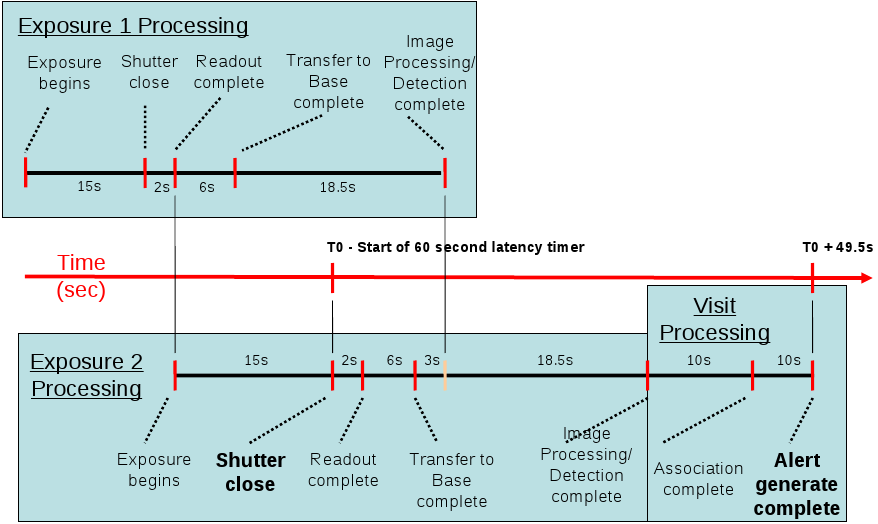
\includegraphics[width=\textwidth]{images/timeline.png}
\caption{A schematic of the alert production time budget.
\label{fig:timeline}}
\end{center}
\end{figure}

Table \ref{tbl:budget} compares the DC3a results with the two
durations in our budget of interest.  We note that, in detail, the
breakdown of our DC3a stages do not neatly map into these duration
categories; for example, there are stages that are done for first
exposure but not the second, and vice version.  In particular, some of
the results from the first exposure is reused for the second.
Nevertheless, a useful rough comparison can be illustrated if we
combine the image processing budgets for each exposure and then take
all production stages (as tagged in table \ref{tbl:ipsdstages},
\Sec{sec:recsummary}) up to and including image subtraction (plus the
time to write out the subtracted image) to constitute image
processing.  (In addition, we will leave out reading in calibration
data assuming this can be done once for the night.)  For association,
we take the remaining stages in IPSD that operate on both exposures
{\it plus} the production stages from AP.  The table breaks the costs
in time between applying science algorithms and I/O (plus the
miscellaneous book-keeping stages).

\begin{table}[htbp]
\centering
\caption{A Comparison of the Alert Production time budget with average
  DC3a costs 
\label{tbl:budget}}
\vspace{\baselineskip}
\begin{tabular}{lc|ccc}
\hline\hline
                           &        & \multicolumn{3}{c}{DC3a Costs}   \\
Budget Category            & Budget & Science    & I/O       & Total   \\
\hline
Image Processing/Detection & 18.5 s & 169.1 s    & 48.3 s    & 217.4 s \\
Association                & 10.0 s &   8.7 s    &  2.8 s    &  11.5 s \\
\hline
\end{tabular}
\end{table}

Clearly, we need to improve the performance of the image processing
part by a factor of ten.  We can understand this challenge better by
comparing these totals with the per-stage costs presented in the
Results section; that is, note:

\begin{itemize}
\item Of the 169 seconds spent on science part of image processing, all
  but 6 seconds are spent on image subtraction.
\item 56\% of the I/O time in support of image processing was spent on
  reading in the template sub-images. 
\item Of the 9 seconds spent on the science part of association, all
  but 2 seconds are spent on ``add-and-detect''.  
\end{itemize}

These results, therefore, suggest that the best strategy for meeting
our time budget must include the following:

\begin{itemize}
\item We must substantially improve the image subtraction algorithm.
  As mentioned previously, we believe that 25\% improvement can come
  simply from tuning configuration parameters.  
\item We must develop better strategies for efficient I/O.  In
  particular, significant gains would be gotten via a more
  embarrassingly parallel I/O access to the template data.
\item Decent gains might also be gotten in improvements to the
  add-and-detect stage.  
\end{itemize}

